\changecolours{ScoutGreen}
\section{Duelo de Paradigmas: ACID vs BASE}

% ------------------------------------------------------------------------------
\twocolframe[title={O Paradigma ACID: Filosofia Pessimista \& Travas},leftcol=7cm,rightcol=7cm]{%
  \alert{Origem: Jim Gray (VLDB, 1981)}\par
  \itemseps[topsepi=1.5mm,itemsepi=2.5mm,labelsep=2mm,leftmargini=4mm]
  \begin{itemize}
    \item Padrão ouro dos sistemas relacionais tradicionais (RDBMS):
    \item \textbf{Atomicidade:} A transação é indivisível (tudo ou nada).
    \item \textbf{Consistência:} Regras de negócio e chaves sempre válidas.
    \item \textbf{Isolamento:} Transações simultâneas não interferem.
    \item \textbf{Durabilidade:} Persistência permanente após commit.
  \end{itemize}
}{%
  \alert{O Gargalo da Abordagem Pessimista}\par
  \itemseps[topsepi=2mm,itemsepi=3mm,labelsep=2mm,leftmargini=4mm]
  \begin{itemize}
    \item O isolamento estrito exige \textbf{travas de leitura e escrita} (\textit{Locks}) e protocolos como \textbf{2PC} (\textit{Two-Phase Commit}).
    \item Sob concorrência massiva, travas geram filas e \textit{deadlocks}.
    \item \textbf{Filosofia:} \textit{``Prefiro travar a requisição a correr o risco de gravar um dado imperfeito.''}
  \end{itemize}
}

% ------------------------------------------------------------------------------
\twocolframe[title={O Paradigma BASE: Filosofia Otimista \& Alta Escala},leftcol=7cm,rightcol=7cm]{%
  \alert{Origem: Werner Vogels \& Dan Pritchett}\par
  \itemseps[topsepi=1.5mm,itemsepi=2.5mm,labelsep=2mm,leftmargini=4mm]
  \begin{itemize}
    \item Criado para sustentar as gigantes da Web (Amazon, Google):
    \item \textbf{BA -- Basically Available:} O sistema continua respondendo mesmo com falhas parciais em nós.
    \item \textbf{S -- Soft State:} O estado dos dados pode mudar com o tempo mesmo sem nova requisição externa.
    \item \textbf{E -- Eventual Consistency:} Réplicas convergem assincronamente para o mesmo valor com o tempo.
  \end{itemize}
}{%
  \alert{A Vantagem da Abordagem Otimista}\par
  \itemseps[topsepi=2mm,itemsepi=3mm,labelsep=2mm,leftmargini=4mm]
  \begin{itemize}
    \item Elimina completamente as travas distribuídas bloqueantes.
    \item Permite vazão de centenas de milhares de escritas por segundo.
    \item \textbf{Filosofia:} \textit{``Prefiro responder em milissegundos e reconciliar os dados assincronamente em segundo plano.''}
  \end{itemize}
}

% ------------------------------------------------------------------------------
\begin{frame}{Duelo dos Paradigmas: ACID vs. BASE Lado a Lado}
  \vspace{-0.3cm}
  \makebox[\linewidth][c]{%
    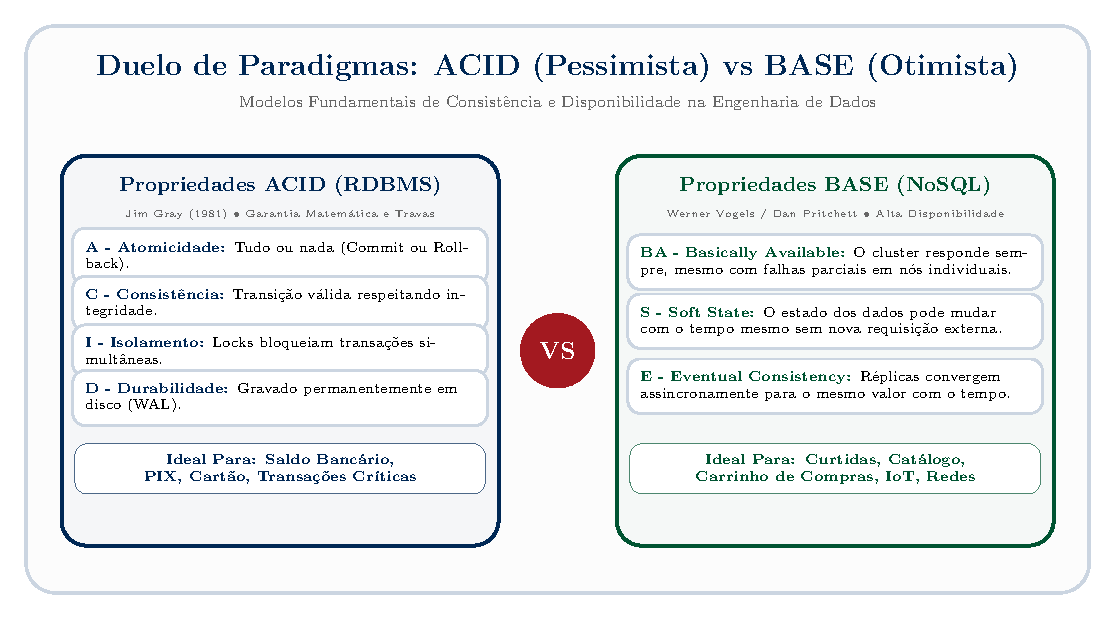
\includegraphics[width=14.0cm,height=4.8cm,keepaspectratio]{figuras/fig_acid_vs_base.pdf}%
  }\par
  \vspace{0.15cm}
  \centering
  {\footnotesize \textbf{Diretriz Arquitetural:} \textcolor{ScoutGreen}{Não existe modelo superior. O bom engenheiro de software escolhe o paradigma de acordo com o domínio de negócio.}}
\end{frame}

% ------------------------------------------------------------------------------
\twocolframe[title={Como Funciona a Consistência Eventual na Prática?},leftcol=7cm,rightcol=7cm]{%
  \alert{O Algoritmo Last-Write-Wins (LWW)}\par
  \itemseps[topsepi=2mm,itemsepi=3mm,labelsep=2mm,leftmargini=4mm]
  \begin{itemize}
    \item Cada escrita recebe um carimbo de tempo físico (\textit{timestamp}).
    \item A versão com maior carimbo sobrescreve versões anteriores.
    \item \textbf{Risco Real:} Desvios de relógio (\textit{Clock Drift}) entre servidores podem descartar escritas legítimas.
  \end{itemize}
}{%
  \alert{Vetores de Versão (Vector Clocks)}\par
  \itemseps[topsepi=2mm,itemsepi=3mm,labelsep=2mm,leftmargini=4mm]
  \begin{itemize}
    \item Cada nó mantém contadores lógicos por registro.
    \item Identifica se uma alteração foi causal ou concorrente.
    \item \textbf{Caso Real (Amazon Dynamo):} O carrinho de compras une itens conflitantes em vez de apagar qualquer um!
  \end{itemize}
}

% ------------------------------------------------------------------------------
\begin{frame}{Matriz Decisória de Negócio: Onde Aplicar Cada Paradigma}
  \vspace{-0.2cm}
  \centering
  \resizebox{0.95\textwidth}{!}{%
  \begin{tabular}{p{4.0cm}p{2.5cm}p{7.5cm}}
    \toprule
    \textbf{Domínio de Negócio} & \textbf{Paradigma} & \textbf{Justificativa Arquitetural} \\
    \midrule
    \textbf{Transferência PIX} & \textcolor{ScoutNavy}{\textbf{ACID / CP}} & O saldo não tolera inconsistência. Gasto duplo gera rombo financeiro. \\
    \addlinespace
    \textbf{Curtidas no TikTok} & \textcolor{ScoutGreen}{\textbf{BASE / AP}} & Perder pequenas contagens em milhões de visualizações é aceitável. \\
    \addlinespace
    \textbf{Carrinho de Compras} & \textcolor{ScoutGreen}{\textbf{BASE / AP}} & Rejeitar o cliente perde a venda. Melhor reconciliar itens depois. \\
    \addlinespace
    \textbf{Vagas SISU / Concursos} & \textcolor{ScoutNavy}{\textbf{ACID / CP}} & Disputas por fração de segundo exigem isolamento estrito. \\
    \bottomrule
  \end{tabular}%
  }
\end{frame}
